\documentclass[preview]{standalone}
%\usepackage{prelude}

%%%%%%%%%%%%%%%%%%%%%%%%%%%%%%%%%%%% PACKAGES %%%%%%%%%%%%%%%%%%%%%%%%%%%%%%%%%%%%%%%%%%

\usepackage{inputenc,fontenc}
\usepackage[a4paper,margin=3cm]{geometry}
\usepackage[english]{babel}
%\usepackage[german]{babel}
%\usepackage[fixlanguage]{babelbib}


\usepackage{bbold}
\usepackage{amsthm}
\usepackage{amsmath}
\usepackage{amssymb} % doteqdot
\usepackage[dvipsnames]{xcolor}
\usepackage{standalone}
\usepackage{tikz}[mode=buildnew]
\usepackage{cite}
\usepackage{xspace}
\usepackage{relsize}
\usepackage{mathtools} % mathclap
%\usepackage{MnSymbol}
\usepackage{hyperref}
\usepackage{url}
\usepackage{listings} % for code
\usepackage[T1]{fontenc} %<
\hypersetup{
	colorlinks,
	citecolor=black,
	filecolor=black,
	linkcolor=black,
	urlcolor=black
}
\usepackage{pgfplots}
\pgfplotsset{compat=1.18}
%\usepackage{courier} %% Sets font for listing as Courier. But also for url and texttt!
\usepackage{listings, xcolor}
\usepackage{graphicx}
\usepackage{subcaption}

\usetikzlibrary{calc}
%\usepackage{xparse} % \newDocumentCommand for multiple optional arguments
%\usepackage{titlecaps}



%%%%%%%%%%%%%%%%%%%%%%%%%%%%%%%%%%%% THEOREMSTYLES %%%%%%%%%%%%%%%%%%%%%%%%%%%%%%%%%%

\theoremstyle{definition}
\newtheorem{definition}{Definition}[section]
\newtheorem{exmp}{Beispiel}[section]
%\AfterEndEnvironment{definition}{\noindent\ignorespaces}

\theoremstyle{theorem}
\newtheorem{theorem}{Satz}[section]
\newtheorem{proposition}{Proposition}[section]
%\AfterEndEnvironment{theorem}{\noindent\ignorespaces}

\theoremstyle{korollary}
\newtheorem{korollary}{Korollar}[section]
%\AfterEndEnvironment{korollary}{\noindent\ignorespaces}


\tikzset{
	mstate/.style={draw, circle, minimum size=.94cm}, 
	gstate/.style={draw, rectangle, minimum size=.8cm},
	varstate/.style={draw,rectangle, rounded corners, minimum size=1}, 
	trans/.style={draw, ->, thick},
	bendtrans/.style={draw, ->, thick, bend left=10},
	bendtransr/.style={draw, ->, thick, bend right=10},
	init/.style={initial, initial distance=6pt, initial text=},
	every loop/.style={min distance=5pt, looseness=8},
	>=latex
}
\usetikzlibrary{automata,positioning}

%auto shift/.style={auto=right,->,
%	to path={ let \p1=(\tikztostart),\p2=(\tikztotarget),
%		\n1={atan2(\y2-\y1,\x2-\x1)},\n2={\n1+180}
%		in ($(\tikztostart.{\n1})!1mm!270:(\tikztotarget.{\n2})$) -- 
%		($(\tikztotarget.{\n2})!1mm!90:(\tikztostart.{\n1})$) \tikztonodes}},

%%%%%%%%%%%%%%%%%%%%%%%%%%%%%%%%%%% MY MACROS %%%%%%%%%%%%%%%%%%%%%%%%%%%%%%%%%%%%%%%%%
%formatting
\newcommand{\comment}[2]{{\color{#1}#2}}
\newcommand{\redcomment}[1]{{\color{red}#1}}
\newcommand{\purpcomment}[1]{{\color{pink}#1}}
\newcommand{\bluecomment}[1]{{\color{blue}#1}}
\newcommand{\mt}[1]{\ensuremath{{#1}}\xspace}
\newcommand{\mynewcommand}[2]{\newcommand{#1}{\mt{#2}}} %% currently not used becaue of ide highlighting
\newcommand{\arr}{\mt{\to}}

%model checking terms
\newcommand{\mimicrel}{\mt{\mathcal{R}}}
\newcommand{\bisimeq}{\mt{\;\!\sim\;\!}}
\newcommand{\simorder}{\mt{\;\!\preceq\;\!}}
\newcommand{\simequiv}{\mt{\;\!\simeq\;\!}} %command already defined
\newcommand{\relts}{\mt{\;\!\bullet_{_{\tiny{TS}}}\;\!}}
\newcommand{\rel}{\mt{\;\!\bullet\;\!}}

%own names
\newcommand{\nm}[1]{#1\xspace}
\newcommand{\mdpN}{\nm{MDP}}
\newcommand{\mdpsN}{\nm{MDPs}}
\newcommand{\viewN}{\nm{view}}
\newcommand{\viewNC}{\nm{View}}
\newcommand{\viewsN}{\nm{views}}
\newcommand{\viewsNC}{\nm{Views}}
\newcommand{\grpfctsubN}{\nm{detached grouping function}}
\newcommand{\grpfctsubNC}{\nm{detached grouping function}}
\newcommand{\grpfctsubNCC}{\nm{Detached Grouping Function}}
\newcommand{\grpfctN}{\nm{grouping function}}
\newcommand{\grpfctNC}{\nm{Grouping function}}
\newcommand{\grpfctNCC}{\nm{Grouping Function}}
\newcommand{\grpfctsN}{\nm{grouping functions}}
\newcommand{\grpfctsNC}{\nm{Grouping functions}}
\newcommand{\grpfctsNCC}{\nm{Grouping Functions}}
\newcommand{\stmimicN}{\nm{state-mimic}}
\newcommand{\stmimicsN}{\nm{state-mimics}}
\newcommand{\stmimickingN}{\nm{state-mimicking}}
\newcommand{\stmimickedN}{\nm{state-mimicked}}
%\newcommand{\chosenphtypeNCC}{\nm{Transition System}}
%\newcommand{\chgphNC}{\nm{Transition system}}
%\newcommand{\chgphN}{\nm{transition system}}
%\newcommand{\chgphsNCC}{\nm{Transition Systems}}
%\newcommand{\chgphsNC}{\nm{Transition systems}}
%\newcommand{\chgphsN}{\nm{transition systems}}
\newcommand{\chgphNCC}{\nm{MDP}}
\newcommand{\chgphNC}{\nm{MDP}}
\newcommand{\chgphN}{\nm{MDP}}
\newcommand{\achgphN}{\nm{an MDP}}
\newcommand{\chgphsNCC}{\nm{MDPs}}
\newcommand{\chgphsNC}{\nm{MDPs}}
\newcommand{\chgphsN}{\nm{MDPs}}
\newcommand{\parllcompN}{\nm{parallel composition}}
\newcommand{\parllcompNC}{\nm{Parallel composition}}
\newcommand{\parllcompNCC}{\nm{Parallel Composition}}
\newcommand{\parllcompsN}{\nm{parallel compositions}}
\newcommand{\parllcompsNC}{\nm{Parallel compositions}}
\newcommand{\parllcompsNCC}{\nm{Parallel Compositions}}
\newcommand{\sccN}{\nm{SCC}}
\newcommand{\sccsN}{\nm{SCCs}}
\newcommand{\bsccN}{\nm{BSCC}}
\newcommand{\bsccsN}{\nm{BSCCs}}
\newcommand{\jgrapht}{\nm{jGraphtT}}

\newcommand{\outactident}{\nm{OutActionsIdent}}

%names
\newcommand{\iffN}{\nm{if and only if}}
\newcommand{\tsN}{\nm{TS}}

%% outactions identical
\newcommand{\outactidentstrong}{\nm{strong}}
\newcommand{\outactidentweak}{\nm{weak}}

% CORE DEFINITIONS
\newcommand{\grpfct}[1][\viewppty]{\mt{F_{#1}}}
\newcommand{\grpfctsub}[1][\viewppty]{\mt{\tilde{F}_{#1}}}
%\newcommand{\grpfctimg}[1]{\mt{{\grpfct}[{#1}]}}
%\newcommand{\fctimg}[2]{\mt{{#1}[{#2}]}}
\newcommand{\eqrelview}{\mt{R}}
\newcommand{\eqclassv}[1][\state]{\mt{\eqclass{#1}{\eqrelview}}}
\newcommand{\eqclasssetv}[1][\states]{\mt{{#1}/\eqrelview}} %OLD: \bigcup_{\state \in \states} \eqclassv
\newcommand{\viewid}{\mt{\mdp}}
\newcommand{\view}[1][\viewppty]{\mt{\viewid_{#1}}}
\newcommand{\imggrp}{\mt{\arbset}}
\newcommand{\imggrpsub}{\mt{X}}
\newcommand{\viewppty}{\mt{\theta}}
\newcommand{\pll}{\mt{\;\!\pllpure\;\!}}
\newcommand{\pllrev}{\mt{\pllpure^{-1}}}
\newcommand{\pllpure}{\mt{||}}
\newcommand{\compselectset}{\mt{Z}}
\newcommand{\compselectpure}{\mt{\pllpure_\compselectset}}
\newcommand{\compselect}{\mt{\;\pllpure_\compselectset\;}}
\newcommand{\remstates}{\mt{\bigcup_{\state \in \states \setminus \states_1}\{\{\state\}\}}}
\newcommand{\nogroupstates}[1][\states_2]{\mt{\bigcup_{\state \in \states \setminus {#1}}\{\{\state\}\}}}
\newcommand{\remelem}{\mt{\bullet}}
\newcommand{\nogroupset}{\mt{\xi}}
\newcommand{\remset}{\mt{\{\remelem\}}}
\newcommand{\gfctpll}{\mt{\grpfct[\pll]}}
\newcommand{\group}{\mt{\top}}
\newcommand{\imggrpbinview}{\mt{\{\remelem, \notppty\}}}
\newcommand{\viewappset}{\mt{\tilde{\states}}}
\newcommand{\hasppty}{\mt{\top}}
\newcommand{\notppty}{\mt{\bot}}
\newcommand{\disregardelem}{\mt{\Delta}}
\newcommand{\disregardelements}{\mt{{\disregardelem_1, \dots, \disregardelem_n}}}



%\newcommand{\mdp}{def}\mdp
%\newcommand{\mdpdef}



% EXAMPLE VIEWS
\newcommand{\pptyatomicprops}{\mt{\atomicprops}}
\newcommand{\pptyinitstates}{\mt{\initstates}}
\newcommand{\pptyinactsetsize}{\mt{|\inacts(\state)|}}
\newcommand{\pptyhasoutact}{\mt{\exists\outact}}
\newcommand{\pptyminoutact}[2]{\mt{#1\leq#2}}
\newcommand{\pptymaxoutact}[2]{\mt{#2\leq#1}}
\newcommand{\pptyspanoutact}[3]{\mt{#1\leq#2\leq#3}}
\newcommand{\pptyoutactsetsize}{\mt{|\outacts(\state)|}}
\newcommand{\pptyoutactsingle}{\mt{|\outacts(\state)|_1}}
\newcommand{\pptystrongoutactident}{\mt{\outacts(\state)_=}}
\newcommand{\pptyweakoutactident}{\mt{\outacts(\state)_\approx}}
\newcommand{\pptyhasinact}{\mt{\exists\inact}}
\newcommand{\pptymininact}[2]{\mt{#1\leq#2}}
\newcommand{\pptymaxinact}[2]{\mt{#2\leq#1}}
\newcommand{\pptyspaninact}[3]{\mt{#1\leq#2\leq#3}}
\newcommand{\pptyinactsingle}{\mt{|\inacts(\state)|_1}}
\newcommand{\pptystronginactident}{\mt{\inacts(\state)_=}}
\newcommand{\pptyweakinactident}{\mt{\inacts(\state)_\approx}}
\newcommand{\pptyparamvalueseq}{\mt{\var = \varval}}
\newcommand{\pptyparamvaluesneq}{\mt{\var \neq \varval}}
\newcommand{\pptyparamdnf}{\mt{VarDNF}}
\newcommand{\pptyparamcnf}{\mt{VarCNF}}
\newcommand{\pptyparamvalueseqopt}{\mt{\var = \varval}}
\newcommand{\pptyparamvalident}{\mt{Var:\varval}}
\newcommand{\pptydistance}{\mt{\distpath}}
\newcommand{\pptydistancerev}{\mt{\distpathrev}}
\newcommand{\pptydistancebi}{\mt{\distpathbi}}
\newcommand{\pptyhascycle}{\mt{\exists\cycle}}
\newcommand{\pptyexactactcycle}{\mt{\{\cycle_{\action,n}\}}}
\newcommand{\pptycycleset}{\mt{\cup{\{\state\}_\cycle}}}
\newcommand{\pptyexactcycle}{\mt{\{\cycle_n\}}}
\newcommand{\pptyscc}{\mt{scc}}
\newcommand{\pptybscc}{\mt{bscc}}
\newcommand{\pptyprop}{\mt{\redcomment{?}}}
\newcommand{\pptyident}{id}


\newcommand{\gfctatomicprops}{\mt{\grpfct[\pptyatomicprops]}}
\newcommand{\gfctinitstates}{\mt{\grpfct[\pptyinitstates]^\hasppty}}
\newcommand{\gfcthasoutaction}{\mt{\grpfct[\pptyhasoutact]^\hasppty}}
\newcommand{\gfctminoutaction}{\mt{\grpfct[\pptyminoutact{\numoutact}{\outact}]^\hasppty}}
\newcommand{\gfctmaxoutaction}{\mt{\grpfct[\pptymaxoutact{\numoutact}{\outact}]^\hasppty}}
\newcommand{\gfctspanoutaction}{\mt{\grpfct[\pptyspanoutact{\numoutactb}{\outact}{\numoutact}]^\hasppty}}
\newcommand{\gfctoutactsetsize}{\mt{\grpfct[\pptyoutactsetsize]}}
\newcommand{\gfctoutactsingle}{\mt{\grpfct[\pptyoutactsingle]^\notppty}}
\newcommand{\gfctstrongoutactident}{\mt{\grpfct[\pptystrongoutactident]}}
\newcommand{\gfctweakoutactident}{\mt{\grpfct[\pptyweakoutactident]}}
\newcommand{\gfcthasinaction}{\mt{\grpfct[\pptyhasinact]^\hasppty}}
\newcommand{\gfctmininaction}{\mt{\grpfct[\pptymininact{\numinact}{\inact}]^\hasppty}}
\newcommand{\gfctmaxinaction}{\mt{\grpfct[\pptymaxinact{\numinact}{\inact}]^\hasppty}}
\newcommand{\gfctspaninaction}{\mt{\grpfct[\pptyspaninact{\numinactb}{\inact}{\numinact}]^\hasppty}}
\newcommand{\gfctinactsetsize}{\mt{\grpfct[\pptyinactsetsize]}}
\newcommand{\gfctinactsingle}{\mt{\grpfct[\pptyinactsingle]^\notppty}}
\newcommand{\gfctstronginactident}{\mt{\grpfct[\pptystronginactident]}}
\newcommand{\gfctweakinactident}{\mt{\grpfct[\pptyweakinactident]}}
\newcommand{\gfctparamvalueseq}{\mt{\grpfct[\pptyparamvalueseq]^\hasppty}}
\newcommand{\gfctparamvaluesneq}{\mt{\grpfct[\pptyparamvaluesneq]^\hasppty}}
\newcommand{\gfctparamdnf}{\mt{\grpfct[\pptyparamdnf]^\hasppty}}
\newcommand{\gfctparamcnf}{\mt{\grpfct[\pptyparamcnf]^\hasppty}}
\newcommand{\gfctparamvalueseqopt}{\mt{\pptyparamvalueseqopt}}
\newcommand{\gfctparamvalident}{\mt{\grpfct[\pptyparamvalident]}}
\newcommand{\gfctdistance}{\mt{\grpfct[\pptydistance]}}
\newcommand{\gfctdistancerev}{\mt{\grpfct[\pptydistancerev]}}
\newcommand{\gfctdistancebi}{\mt{\grpfct[\pptydistancebi]}}
\newcommand{\gfcthascycle}{\mt{\grpfct[\pptyhascycle]}}
\newcommand{\gfctexactcycle}{\mt{\grpfct[\pptyexactcycle]}}
\newcommand{\gfctcycleset}{\mt{\grpfct[\pptycycleset]}}
\newcommand{\gfctexactactcycle}{\mt{\grpfct[\pptyexactactcycle]}}
\newcommand{\gfctscc}{\mt{\grpfct[\pptyscc]}}
\newcommand{\gfctbscc}{\mt{\grpfct[\pptybscc]}}
\newcommand{\gfctprop}{\mt{\grpfct[\pptyprop]}}
\newcommand{\gfctident}{\mt{\grpfct[\pptyident]}}

\newcommand{\gfctsubatomicprops}{\mt{\grpfctsub[\pptyatomicprops]}}
\newcommand{\gfctsubinitstates}{\mt{\grpfctsub[\pptyinitstates]^\hasppty}}
\newcommand{\gfctsubhasoutaction}{\mt{\grpfctsub[\pptyhasoutact]^\hasppty}}
\newcommand{\gfctsubminoutaction}{\mt{\grpfctsub[\pptyminoutact{\numoutact}{\outact}]^\hasppty}}
\newcommand{\gfctsubmaxoutaction}{\mt{\grpfctsub[\pptymaxoutact{\numoutact}{\outact}]^\hasppty}}
\newcommand{\gfctsubspanoutaction}{\mt{\grpfctsub[\pptyspanoutact{\numoutactb}{\outact}{\numoutact}]^\hasppty}}
\newcommand{\gfctsuboutactsetsize}{\mt{\grpfctsub[\pptyoutactsetsize]}}
\newcommand{\gfctsuboutactsingle}{\mt{\grpfctsub[\pptyoutactsingle]^\notppty}}
\newcommand{\gfctsubstrongoutactident}{\mt{\grpfctsub[\pptystrongoutactident]^\hasppty}}
\newcommand{\gfctsubweakoutactident}{\mt{\grpfctsub[\pptyweakoutactident]^\hasppty}}
\newcommand{\gfctsubhasinaction}{\mt{\grpfctsub[\pptyhasinact]}}
\newcommand{\gfctsubmininaction}{\mt{\grpfctsub[\pptymininact{\numinact}{\inact}]}}
\newcommand{\gfctsubmaxinaction}{\mt{\grpfctsub[\pptymaxinact{\numinact}{\inact}]}}
\newcommand{\gfctsubspaninaction}{\mt{\grpfctsub[\pptyspaninact{\numinactb}{\inact}{\numinact}]}}
\newcommand{\gfctsubinactsetsize}{\mt{\grpfctsub[\pptyinactsetsize]^\hasppty}}
\newcommand{\gfctsubinactsingle}{\mt{\grpfctsub[\pptyinactsingle]^\notppty}}
\newcommand{\gfctsubstronginactident}{\mt{\grpfctsub[\pptystronginactident]}}
\newcommand{\gfctsubweakinactident}{\mt{\grpfctsub[\pptyweakinactident]}}
\newcommand{\gfctsubparamvalueseq}{\mt{\grpfctsub[\pptyparamvalueseq]^\hasppty}}
\newcommand{\gfctsubparamvaluesneq}{\mt{\grpfctsub[\pptyparamvaluesneq]^\hasppty}}
\newcommand{\gfctsubparamdnf}{\mt{\grpfctsub[\pptyparamdnf]^\hasppty}}
\newcommand{\gfctsubparamcnf}{\mt{\grpfctsub[\pptyparamcnf]^\hasppty}}
\newcommand{\gfctsubparamvalueseqopt}{\mt{\pptyparamvalueseqopt}}
\newcommand{\gfctsubparamvalident}{\mt{\grpfctsub[\pptyparamvalident]}}
\newcommand{\gfctsubdistance}{\mt{\grpfctsub[\pptydistance]}}
\newcommand{\gfctsubdistancerev}{\mt{\grpfctsub[\pptydistancerev]}}
\newcommand{\gfctsubdistancebi}{\mt{\grpfctsub[\pptydistancebi]}}
\newcommand{\gfctsubhascycle}{\mt{\grpfctsub[\pptyhascycle]^\hasppty}}
\newcommand{\gfctsubexactcycle}{\mt{\grpfctsub[\pptyexactcycle]}}
\newcommand{\gfctsubcycleset}{\mt{\grpfctsub[\pptycycleset]}}
\newcommand{\gfctsubexactactcycle}{\mt{\grpfctsub[\pptyexactactcycle]}}
\newcommand{\gfctsubscc}{\mt{\grpfctsub[\pptyscc]}}
\newcommand{\gfctsubbscc}{\mt{\grpfctsub[\pptybscc]}}
\newcommand{\gfctsubprop}{\mt{\grpfctsub[\pptyprop]}}
\newcommand{\gfctsubident}{\mt{\grpfctsub[\pptyident]}}


\newcommand{\viewatomicprops}{\mt{\view[\pptyatomicprops]}}
\newcommand{\viewinitstates}{\mt{\view[\pptyinitstates]^\hasppty}}
\newcommand{\viewhasoutaction}{\mt{\view[\pptyhasoutact]^\hasppty}}
\newcommand{\viewminoutaction}{\mt{\view[\pptyminoutact{\numoutact}{\outact}]^\hasppty}}
\newcommand{\viewmaxoutaction}{\mt{\view[\pptymaxoutact{\numoutact}{\outact}]^\hasppty}}
\newcommand{\viewspanoutaction}{\mt{\view[\pptyspanoutact{\numoutactb}{\outact}{\numoutact}]^\hasppty}}
\newcommand{\viewoutactsetsize}{\mt{\view[\pptyoutactsetsize]}}
\newcommand{\viewoutactsingle}{\mt{\view[\pptyoutactsingle]^\notppty}}
\newcommand{\viewstrongoutactident}{\mt{\view[\pptystrongoutactident]}}
\newcommand{\viewweakoutactident}{\mt{\view[\pptyweakoutactident]}}
\newcommand{\viewhasinaction}{\mt{\view[\pptyhasinact]^\hasppty}}
\newcommand{\viewmininaction}{\mt{\view[\pptymininact{\numinact}{\inact}]^\hasppty}}
\newcommand{\viewmaxinaction}{\mt{\view[\pptymaxinact{\numinact}{\inact}]^\hasppty}}
\newcommand{\viewspaninaction}{\mt{\view[\pptyspaninact{\numinactb}{\inact}{\numinact}]^\hasppty}}
\newcommand{\viewinactsetsize}{\mt{\view[\pptyinactsetsize]}}
\newcommand{\viewinactsingle}{\mt{\view[\pptyinactsingle]^\notppty}}
\newcommand{\viewstronginactident}{\mt{\view[\pptystronginactident]}}
\newcommand{\viewweakinactident}{\mt{\view[\pptyweakinactident]}}
\newcommand{\viewparamvalueseq}{\mt{\view[\pptyparamvalueseq]}}
\newcommand{\viewparamvaluesneq}{\mt{\view[\pptyparamvaluesneq]}}
\newcommand{\viewparamdnf}{\mt{\view[\pptyparamdnf]^\hasppty}}
\newcommand{\viewparamcnf}{\mt{\view[\pptyparamcnf]^\hasppty}}
\newcommand{\viewparamvalueseqopt}{\mt{\pptyparamvalueseqopt}}
\newcommand{\viewparamvalident}{\mt{\view[\pptyparamvalident]}}
\newcommand{\viewdistance}{\mt{\view[\pptydistance]}}
\newcommand{\viewdistancerev}{\mt{\view[\pptydistancerev]}}
\newcommand{\viewdistancebi}{\mt{\view[\pptydistancebi]}}
\newcommand{\viewhascycle}{\mt{\view[\pptyhascycle]}}
\newcommand{\viewexactcycle}{\mt{\view[\pptyexactcycle]}}
\newcommand{\viewcycleset}{\mt{\view[\pptycycleset]}}
\newcommand{\viewexactactcycle}{\mt{\view[\pptyexactactcycle]}}
\newcommand{\viewscc}{\mt{\view[\pptyscc]}}
\newcommand{\viewbscc}{\mt{\view[\pptybscc]}}
\newcommand{\viewprop}{\mt{\view[\pptyprop]}}
\newcommand{\viewident}{\mt{\view[\pptyident]}}

%\newcommand{\viewatomicprops}{\mt{\view[\atomicprops]}}
%\newcommand{\viewinitstates}{\mt{\view[\initstates]}}
%\newcommand{\viewhasoutaction}{\mt{\view[\pptyhasoutact]}}
%\newcommand{\viewminoutaction}{\mt{\view[\pptyminoutact{\numoutact}{\outact}]}}
%\newcommand{\viewmaxoutaction}{\mt{\view[\pptymaxoutact{\numoutact}{\outact}]}}
%\newcommand{\viewspanoutaction}{\mt{\view[\pptyspanoutact{\numoutactb}{\outact}{\numoutact}]}}
%\newcommand{\viewoutactsetsize}{\mt{\view[\pptyoutactsetsize]}}
%\newcommand{\viewoutactsingle}{\mt{\view[\pptyoutactsingle]}}
%\newcommand{\viewstrongoutactident}{\mt{\view[\outacts(\state)_=]}}
%\newcommand{\viewweakoutactident}{\mt{\view[\outacts(\state)_\approx]}}
%\newcommand{\viewhasinaction}{\mt{\view[\pptyhasinact]}}
%\newcommand{\viewmininaction}{\mt{\view[\pptymininact{\numinact}{\inact}]}}
%\newcommand{\viewmaxinaction}{\mt{\view[\pptymaxinact{\numinact}{\inact}]}}
%\newcommand{\viewspaninaction}{\mt{\view[\pptyspaninact{\numinactb}{\inact}{\numinact}]}}
%\newcommand{\viewinactsetsize}{\mt{\view[\pptyinactsetsize]}}
%\newcommand{\viewinactsingle}{\mt{\view[\pptyinactsingle]}}
%\newcommand{\viewstronginactident}{\mt{\view[\inacts(\state)_=]}}
%\newcommand{\viewweakinactident}{\mt{\view[\inacts(\state)_\approx]}}
%\newcommand{\viewparamvalueseq}{\mt{\view[\var = \varval]}}
%\newcommand{\viewparamvaluesneq}{\mt{\view[\var \neq \varval]}}
%\newcommand{\viewparamdnf}{\mt{\view[VarDNF]}}
%\newcommand{\viewparamcnf}{\mt{\view[VarCNF]}}
%\newcommand{\viewparamvalident}{\mt{\view[\pptyparamvalident]}}
%\newcommand{\viewdistance}{\mt{\view[\pptydistance]}}
%\newcommand{\viewhascycle}{\mt{\view[\exists\cycle]}}
%\newcommand{\viewexactcycle}{\mt{\view[\pptyexactcycle]}}
%\newcommand{\viewcycleset}{\mt{\view[\pptycycleset]}}
%\newcommand{\viewexactactcycle}{\mt{\view[\pptyexactactcycle]}}
%\newcommand{\viewscc}{\mt{\view[scc]}}
%\newcommand{\viewbscc}{\mt{\view[bscc]}}

%actions
\newcommand{\numoutact}{\mt{n}}
\newcommand{\numoutactb}{\mt{m}}
\newcommand{\numinact}{\mt{n}}
\newcommand{\numinactb}{\mt{m}}

\newcommand{\predmaxoutact}[1][\numoutact]{\mt{Q_{\outact\leq#1}(\state,\state_1, \dots, \state_{#1+1})}}
\newcommand{\predminoutact}[1][\numoutact]{\mt{Q_{#1\leq\outact}(\state,\state_1, \dots, \state_{#1})}}
\newcommand{\formoutact}[1][\state]{\mt{C_{#1,\outact}}}
\newcommand{\predmaxinact}[1][\numinact]{\mt{Q_{\inact\leq#1}(\state,\state_1, \dots, \state_{#1+1})}}
\newcommand{\predmininact}[1][\numinact]{\mt{Q_{#1\leq\inact}(\state,\state_1, \dots, \state_{#1})}}

\newcommand{\outact}[1][\action]{\mt{\overrightarrow{#1}}}
\newcommand{\outacts}{\mt{\overrightarrow{\actions}}}
\newcommand{\inact}{\mt{\overleftarrow{\action}}}
\newcommand{\inacts}[1][\action]{\mt{\overleftarrow{#1}}}

%%Parameters
\newcommand{\vars}[1][\mdp]{\mt{V\!ar_{#1}}}
\newcommand{\var}{\mt{x}}
\newcommand{\varstate}[1][]{\mt{\var_{\state#1}}}
\newcommand{\varval}{\mt{a}}
\newcommand{\vareval}[1][\mdp]{\mt{V\!arEval_{#1}}}
\newcommand{\varevalimg}[1][\mdp]{\mt{\vareval[#1][\states,\vars]}}
\newcommand{\varevalimgset}{\mt{\arbset}}
\newcommand{\someparam}{\mt{\tilde{x}}}
\newcommand{\eqorneq}{\mt{\;\doteqdot\;}}
\newcommand{\varstyle}[2]{\mt{\langle#1,#2\rangle}}




%\makeatletter
%\newcommand{\overleftrightsmallarrow}{\mathpalette{\overarrowsmall@\leftrightarrowfill@}}
%\newcommand{\overrightsmallarrow}{\mathpalette{\overarrowsmall@\rightarrowfill@}}
%\newcommand{\overleftsmallarrow}{\mathpalette{\overarrowsmall@\leftarrowfill@}}
%\newcommand{\overarrowsmall@}[3]{%
%	\vbox{%
%		\ialign{%
%			##\crcr
%			#1{\smaller@style{#2}}\crcr
%			\noalign{\nointerlineskip}%
%			$\m@th\hfil#2#3\hfil$\crcr
%		}%
%	}%
%}
%\def\smaller@style#1{%
%	\ifx#1\displaystyle\scriptstyle\else
%	\ifx#1\textstyle\scriptstyle\else
%	\scriptscriptstyle
%	\fi
%	\fi
%}
%\makeatother
%\newcommand{\te}[1]{\overleftrightsmallarrow{#1}}

% Distance
\newcommand{\fctdist}{\mt{distance}}
\newcommand{\fctdistdefault}{\mt{\fctdist(\chgph, \smstates, \grandist)}}
\newcommand{\distval}{\mt{d}}
\newcommand{\grandist}{\mt{n}}
\let\path\oldpath
\newcommand{\path}{\mt{P}}
\newcommand{\pathbi}{\mt{\bar{\path}}}
\newcommand{\pathsecfull}{\mt{(\state_0, \action_0, \state_1, \action_1, \dots, \action_{n}, \state_{n+1})}}
\newcommand{\lenpath}{\mt{len}}
\newcommand{\pfirst}{\mt{first}}
\newcommand{\plast}{\mt{last}}
\newcommand{\pathset}{\mt{\path_\chgph}}
\newcommand{\pathbiset}{\mt{\pathbi_\chgph}}
\newcommand{\distpath}{\mt{\overrightarrow{dist}}}
\newcommand{\distpathrev}{\mt{\overleftarrow{dist}}}
\newcommand{\distpathbi}{\mt{\overline{dist}}}
%Cycles
\newcommand{\cyclesecfull}{\mt{(\state_0, \action_0, \state_1, \action_1, \dots, \action_{n-1}, \state_0)}}
\newcommand{\fctfindcycles}{\mt{findCycles}}
\newcommand{\cycle}{\mt{C}}
\newcommand{\cycleset}{\mt{\cycle_{\mdp, n}}}
\newcommand{\lencycle}{\mt{len}}
% strongly connected components
\newcommand{\scc}{\mt{T}}
\newcommand{\setscc}{\mt{SCC_{\chgph,n}}}
\newcommand{\setbscc}{\mt{BSCC_{\chgph,n}}}

% properties
\newcommand{\propfct}{\mt{f}}

% all Systems
\newcommand{\chgph}{\mt{\mdp}}
\newcommand{\chgphtuple}{\mt{\mdptuple}}
\newcommand{\chgphtupledist}{\mt{\mdptupledist}}

\newcommand{\states}{\mt{S}}
\newcommand{\actions}{\mt{Act}}
\newcommand{\atomicprops}{\mt{AP}}
\newcommand{\labelingfct}{\mt{L}}
\newcommand{\init}{\mt{\initdistrib}} % use MDP % refers to the underlying set
\newcommand{\trans}{\mt{\probtfunc}} % use MDP % refers to the underlying set
\newcommand{\smstates}{\mt{\tilde{\states}}}


\newcommand{\state}{\mt{s}}
\newcommand{\action}{\mt{\alpha}}
\newcommand{\actionb}{\mt{\beta}}
\newcommand{\actionc}{\mt{\gamma}}
\newcommand{\smstate}{\mt{\tilde{\state}}}



% transition sysstems
\newcommand{\ts}{\mt{TS}}
\newcommand{\transitionrel}{\mt{\longrightarrow}}
\newcommand{\initstates}{\mt{I}}
\newcommand{\transitionsystem}{\mt
	{(\states, \actions, \transitionrel, \initstates, \atomicprops, \labelingfct)}
}
\newcommand{\tstupledist}{\mt{(\states', \actions',\transitionrel', \initstates', \labelingfct')}}


%Markov chains and MDP
\newcommand{\mdp}{\mt{\autm}}
\newcommand{\mdptuple}{\mt{(\states, \actions, \probtfunc, \initdistrib, \atomicprops, \labelingfct)}}
\newcommand{\mdptupledist}{\mt{(\states', \actions', \probtfunc', \initdistrib', \atomicprops', \labelingfct')}}
\newcommand{\autm}{\mt{\mathcal{M}}}
\newcommand{\probtfunc}{\mt{\textbf{P}}}
\newcommand{\initdistrib}{\mt{\iota_{init}}}


%maths
\newcommand{\powerset}[1]{\mt{\mathcal{P}(#1)}}
\newcommand{\eqclass}[2]{\mt{[#1]_{#2}}}%{\mt{#1 / #2}}
\newcommand{\impr}{\mt{\hspace{3mm}\Rightarrow\hspace{2mm}}}
\newcommand{\impl}{\mt{\hspace{3mm}\Leftarrow\hspace{2mm}}}
\newcommand{\natnums}{\mt{\mathbb{N}}} 
\newcommand{\realnums}{\mt{\mathbb{R}}}
\newcommand{\intmodn}[1][n]{\mt{\mathbb{Z}_{#1}}}
\newcommand{\arbset}{\mt{M}}
\newcommand{\bigsum}[2][]{\mt{\mathlarger{\sum}_{#2}^{#1}}}
\newcommand{\bbigsum}[2][]{\mt{\mathlarger{\mathlarger{\sum}}_{#2}^{#1}}}
\newcommand{\invimage}[2]{#1^{\mt{-1}(#2)}}
\newcommand{\img}{\mt{Img}}
\newcommand{\cond}{\mt{\,|\,}}

%tickz
%% \definecolor{darkred}{RGB}{196, 42, 42}

%implementation
\newcommand{\pmcvis}{\nm{PMC-Vis}}



\begin{document}

\section{Preliminaries} \label{ch:prelim}

%\subsection{Transition Systems}
\viewsNC will be defined on \chgphsN. Instead of directly providing the definition of \achgphN we will consider less powerful classes of models to represent systems that are extended by \chgphsN.

Firstly we will consider \emph{transition systems}. Transition systems are basically digraphs consisting of \emph{states} and \emph{transitions} in place of nodes and edges. A state describes some information about a system at a certain moment of its behavior, a transition the evolution from one state to another. We will use transition systems with \emph{action names} and \emph{atomic propositions} for states as in \cite{Baier2008}.

\begin{definition}[\!{\cite{Baier2008}, Definition 2.1.}]
	A \emph{transition system} TS is a tuple \transitionsystem where
	\begin{itemize}
		\item \states is a set of states,
		\item \actions is a set of actions,
		\item $\transitionrel \subseteq \states \times \actions \times \states$ is transition relation,
		\item $\initstates \subseteq \states$ is a set of initial states,
		\item \atomicprops is a set of atomic propositions, and
		\item $\labelingfct : \states \to \powerset{\atomicprops}$
	\end{itemize}
\end{definition}

%Considering a traffic light displaying green could be considered as one state whereas displaying red could be another one. Transitions model the progression of the system from one state to another one. Sticking to the example of the traffic light a transition could model the switch from state green light being displayed to the state of red light being displayed. There are several variants of transitions systems. 



A transition system is called \emph{finite} if \states, \atomicprops and \labelingfct are finite. Actions are used for communication between processes. We denote them with Greek letters ($\alpha, \beta, \gamma, \dots$). Atomic propositions are simple facts about states. For instance "x is greater than 20" or "red and yellow light are on" could be atomic propositions. We will denote atomic propositions with arabic letters ($a,b,c,\dots$). They are assigned to a state by a labeling function \labelingfct.

The intuitive behavior of transition systems is as follows. The evolution of a transition system starts in some state $\state \in \initstates$. If the set of \initstates of initial states is empty the transition system has no behavior at all. From the initial state the transition system evolves according to the transition relation \transitionrel. The evolution ends in a state that has no outgoing transitions. For every state there may be several possible transitions to be taken. The choice of which one is take is done nondeterministically. That is the outcome of the selection can not be know a priori. It is especially not following any probability distribution. Hence there can not be made any statement about the likelihood of a transition being selected.

In contrast with \emph{Markov Chains} this nondeterministic behavior is replaced with a probabilistic one. That is for every state there exists a probability distribution that describes the chance of a transition being selected. There are no actions and there is no nondeterminism in Markov Chains.
%\redcomment{NOTES BEGIN}
%\begin{itemize}
%	\item Markov Chain (MC)
%	\item transition systems to markov chains: nondeterministic choices replaced by probablistic
%	\item successor chosen according to probability distribution
%	\item distribution only dependent on current state \state (not path)
%	\item system evolution not dependent on history but only current state $\to$ \emph{memoryless property}
%\end{itemize}
%
%\redcomment{NOTES END}

\begin{definition}[\!{\cite{Baier2008}, Definition 10.1.}]
	A \emph{(discrete-time) Markov chain} is a tuple $\autm = (\states, \probtfunc, \initdistrib, \atomicprops, \labelingfct)$ where 
	\begin{itemize}
		\item \states is a countable, nonempty set of states,
		\item $\probtfunc : \states \times \states \to [0,1]$ is the \emph{transition probability function}, such that for all states \state:
		\begin{center}
			$\bbigsum{\state' \in \states}\probtfunc(\state,\states') = 1$.	
		\end{center}
		\item $\initdistrib : \states \to [0,1]$ is the \emph{initial distribution}, such that $\mathlarger{\sum_{\state \in \states}} \initdistrib(\state) = 1$, and
		\item \atomicprops is a set of atomic propositions and,
		\item $\labelingfct : \states \to \powerset{\atomicprops}$ a labeling function.		
	\end{itemize}
\end{definition}

A Markov Chain (MC) \autm is called \emph{finite} if \states and \atomicprops are finite. \redcomment{For finite \autm, the \emph{size} of \autm, denoted \emph{size}(\autm),  is the number of states plus the number of pairs $(\state, \state') \in \states \times \states$ with $\probtfunc(\state, \state') > 0.$ OMIT??}

%It is important to note that Markov Chains are memoryless in the sense that the system evolution is not dependent on the history of only on the current state. That is the evolution of the system does not depend on the sequence of so far traversed states with the transitions. 

The probability function \probtfunc specifies for each state \state the probability $\probtfunc(\state,\state')$ of moving from \state to \state' in one step. The constraint put on \probtfunc in the second item ensures that \probtfunc is a probability distribution. The value $\initdistrib(\state)$ specifies the likelihood that the system evolution starts in \state. All states \state with $\initdistrib(\state) > 0$ are  considered \emph{initial states}. States \state' with $\probtfunc(\state, \state') > 0$ are viewed as possible successors of the state \state. The operational behavior is as follows. An initial state $\state_0$ is yielded by the initial distribution \initdistrib. Afterwards in each state a transition is yielded at random according to the probability distribution \probtfunc in that state.
%\begin{itemize}
%	\redcomment{\item has no actions \\ "As compositional approaches for Markov models are outside the scope of this monograph,
%	actions are irrelevant in this chapter and are therefore omitted."}
%\end{itemize}

%\redcomment{NOTES BEGIN}
%\begin{itemize}
%	\item Probability Function \probtfunc specifies for each state \state the probability \probtfunc(\state,\state') of moving from \state to \state' in one step.
%	\item constraint on \probtfunc ensures that \probtfunc is distribution
%	\item \initdistrib(\state) specifies system evolution starts in \state
%	\item states \state with $\initdistrib(\state) > 0$ are  considered \emph{initial states}
%	\item states \state' with $\probtfunc(\state, \state') > 0$ are view as possible successors of \state
%	\item has no actions \\ "As compositional approaches for Markov models are outside the scope of this monograph,
%	actions are irrelevant in this chapter and are therefore omitted."
%\end{itemize}
%
%\redcomment{NOTES END}


%\subsection{Markov Decision Process} 

%\redcomment{NOTES BEGIN}
The disadvantage of Markov Chains is that they do not enable process intercommunication and do not permit nondeterminism, but only probabilistic evolution. \emph{Markov Decision Processes} (\mdpsN) permit both probabilistic and nondeterministic choices. An \mdpN thereby is a model that somewhat merges the concept of transition systems with the concept of Markov chains. 
%\begin{itemize}
%	\item probabilistic choices: possible outcomes for of randomized actions -> requires statistical experiments to obtain adequate distributions that model average behavior of the environment
%	\item information not available or guarantee about system properties is required -> nondeterminism
%	\item Another example: randomized distributed algorithms. Non-determinism: interleaving behavior: nondeterministic choice which process, probabilistic: have rather restricted set of actions that have a random nature
%	\item used for abstraction in markov chains: states grouped by \atomicprops and have a wide range of transition probabilities -> essentially nondeterminism -> transition probabilities are replaced by nondeterminism		
%\end{itemize}
%
%\redcomment{NOTES END}
%\redcomment{NOTES BEGIN}
%
%\begin{itemize}
%	\item Markov decision process (MDP) 
%	\item idea: Adding nondeterminism to markov chains. MDPs permit both probabilistic and nondeterministic choices 
%	\item probabilistic choices: possible outcomes for of randomized actions -> requires statistical experiments to obtain adequate distributions that model average behavior of the environment
%	\item information not available or guarantee about system properties is required -> nondeterminism
%	\item Another example: randomized distributed algorithms. Non-determinism: interleaving behavior: nondeterministic choice which process, probabilistic: have rather restricted set of actions that have a random nature
%	\item used for abstraction in markov chains: states grouped by \atomicprops and have a wide range of transition probabilities -> essentially nondeterminism -> transition probabilities are replaced by nondeterminism		
%\end{itemize}

%\redcomment{NOTES END}

\begin{definition}[\!{\cite{Baier2008}, Definition 10.81.}]
	A \emph{Markov decision process} (\mdpN) is a tuple $\mdp = \mdptuple$ where
	\begin{itemize}
		\item \states is a countable set of states,
		\item \actions is a set of actions,
		\item $\probtfunc : \states \times \actions \times \states \to [0,1]$ is the transition probability function such that for all states $\state \in \states$ and actions $\action \in \actions$:
		\begin{center}
			$\bbigsum{\state' \in \states}\probtfunc(\state,\action,\state') \in \{0,1\}$,
		\end{center}
		\item $\initdistrib : \states \to [0,1]$ is the initial distribution such that $\sum_{\state \in \states} \initdistrib(\state) = 1$,
		\item \atomicprops is  a set of atomic propositions and
		\item $\labelingfct : \states \to \powerset{\atomicprops}$ a labeling function.
	\end{itemize}
	An action \action is \emph{enabled} in state \state if and only if $\sum_{\state' \in \states} \probtfunc(\state,\action,\state') = 1$. Let $\actions(\state)$ denote the set of enabled actions in \state. For any state $\state \in \states$, it is required that $\actions(\state) \neq \emptyset$. Each state \state' for which $\probtfunc(\state,\action,\state') > 0$ is called an \emph{\action-successor} of \state.
\end{definition}

%It adds probabilistic choices to transition systems or add nondeterminism to Markov chains. Probabilistic choices may be used to model the (probabilistic) behavior of the environment. But to do so statistical experiments are required to obtain adequate distributions that model the average behavior of the environment. If this information is not available too hard to obtain, or a guarantee about system properties is required nondeterminism is the natural option for modeling in these cases. Further usecases of \mdpsN are randomized distributed algorithms and abstraction in Markov chains. Randomized distributed algorithms are nondeterministic because there is a nondeterministic choice which process performs the next step and randomized because they have rather restricted set of actions that have a random nature. Abstraction in Markov chains can be feasible if states have been grouped by \atomicprops and and have a wide range of transition probabilities. If that is the case selection of a transition is rather non deterministic and thereby can be abstracted with an \mdpN by replacing the probabilities with nondeterminism.

An \mdpN is called \emph{finite} if \states, \actions and \atomicprops are finite.The transition probabilities $\probtfunc(\state, \action, t)$ can be arbitrary real numbers in $[0,1]$ (that sum up to 1 or 0 for fixed \state and \action). For algorithmic purposes they are assumed to be rational.  The unique initial distribution \initdistrib could be generalized to set of \initdistrib with nondeterministic choice at the beginning. For sake of simplicity there is just one single distribution. The operational behavior is as follows. A starting state $\state_0$ yielded by \initdistrib with $\initdistrib(\state_0) > 0$. From there on nondeterministic choice of enabled action takes place followed by a probabilistic choice of a state. The action fixed in the step of nondeterministic selection. Any Markov chain is an \mdpN in which for every state \state, $\actions(\state)$ is a singleton set. Conversely an \mdpN with the property of $\outacts(\state) = 1$ is a Markov chain. Thus Markov chains are a proper subset of Markov decision processes.


For convenience for $\state_1, \state_2 \in \states$ and $\action \in \actions$ we will write $(\state_1, \action, \state_2) \in \probtfunc$ \iffN $\probtfunc(\state_1, \action, \state_2) > 0$, that is to say if there is a non-zero probability of evolving from state $\state_1$ to state $\state_2$ with action \action. Analogously we will write $\state \in \initdistrib$ \iffN is an initial state ($\initdistrib(\state) > 0$). 
We define $\outacts(\state) := \{\action \mid (\state,\action,\smstate) \in \trans\}$ for $\state \in \states$. For $\state \in \states$ we call an element of $\outacts(\state)$ outgoing action of \state. We say a state has an outgoing action \action if $\action \in \outacts(\state)$. We use analogous definition and terminology for incoming actions \inacts. 

\begin{exmp}
In Figure \ref{fig:exampleMdp} we see an graphical representation of an \mdpN. For this \mdpN it is $\states = \{\state_1, \state_2, \state_3, \state_4, \state_5, \state_6\}$, $\actions = \{\action, \actionb, \actionc\}$, $\atomicprops = \{a,b\}$. In Table \ref{tab:atomicpropsandlabelingfunction} we see the values for \labelingfct, \initdistrib and \trans.

\begin{table}[h!]
	\parbox{.45\linewidth}{
		\begin{center}
%			
			\begin{tabular}{c|c|c} % <-- Alignments: 1st column left, 2nd middle and 3rd right, with vertical lines in between
				State & $\labelingfct(\state_i)$ & $\initdistrib(\state_i)$\\		
				\hline
				$\state_1$ & $\emptyset$ & $0.7$\\
				$\state_2$ & $\{a\}$ & $0$\\
				$\state_3$ & $\{a,b\}$ & $0.2$\\
				$\state_4$ & $\{b\}$ & $0.1$\\
				$\state_5$ & $\{a\}$ & $0$\\
				$\state_6$ & $\{b\}$ & $0$\\			
			\end{tabular}
		\end{center}
}
%\hspace{10mm}
\parbox{.45\linewidth}{
		\begin{center}
%			\caption{Your first table.}
%			\label{tab:trans}
			\begin{tabular}{c|c} % <-- Alignments: 1st column left, 2nd middle and 3rd right, with vertical lines in between
				$t \in \states \times \actions \times \states$ & $\trans(t)$\\		
				\hline
				$(\state_1,\action, \state_2)$ & $0.5$\\
				$(\state_1,\action, \state_4)$ & $1$\\
				$(\state_2,\actionb, \state_2)$ & $0.6$\\
				$(\state_2,\actionb, \state_6)$ & $0.4$\\
				$(\state_2,\actionc, \state_1)$ & $1$\\
				$(\state_3,\actionb, \state_3)$ & $0.4$\\
				$(\state_3,\actionb, \state_2)$ & $0.6$\\
				$(\state_3,\actionc, \state_1)$ & $0.8$\\
				$(\state_3,\actionc, \state_4)$ & $0.2$\\
				$(\state_4,\action, \state_4)$ & $0.5$\\
				$(\state_4,\actionc, \state_4)$ & $1$\\
				$(\state_4,\action, \state_3)$ & $0.5$\\
				$(\state_5,\actionb, \state_5)$ & $1$\\
				$(\state_6,\action, \state_6)$ & $1$\\				
			\end{tabular}
		\end{center}
	}
	\caption{Labeling Function, initial distribution and transition probability function of \mdpN in Figure \ref{fig:exampleMdp}. Omitted values of $\trans(t)$ are meant to be zero.}
	\label{tab:atomicpropsandlabelingfunction}
\end{table}

We will declare \mdpsN by only providing its graphical representation. For this the sets $\states, \actions, \atomicprops$ are assumed to be minimal. That is, they contain no more elements than displayed in the graphical representation. Mostly we will use simplified graphical representations of \mdpsN. In these we will omit information. If actions are omitted, it is assumed that each transition $t \in \trans$ has a distinct action. If probabilities are omitted for each state it is assumed the uniform distribution on each set of outgoing transitions with the same action. If the initial distribution is omitted, it is assumed to be the uniform distribution. If atomic propositions are omitted it is assumed that the set of atomic propositions is empty and every state is mapped to the empty set by the labeling function. The purpose of simplified representations is to focus on and only show relevant information. The remaining information is considered irrelevant in these cases.

\begin{figure}[!htb]
	\centering \documentclass[tikz,preview]{standalone}
%\usepackage{prelude}

%%%%%%%%%%%%%%%%%%%%%%%%%%%%%%%%%%%% PACKAGES %%%%%%%%%%%%%%%%%%%%%%%%%%%%%%%%%%%%%%%%%%

\usepackage{inputenc,fontenc}
\usepackage[a4paper,margin=3cm]{geometry}
\usepackage[english]{babel}
%\usepackage[german]{babel}
%\usepackage[fixlanguage]{babelbib}


\usepackage{bbold}
\usepackage{amsthm}
\usepackage{amsmath}
\usepackage{amssymb} % doteqdot
\usepackage[dvipsnames]{xcolor}
\usepackage{standalone}
\usepackage{tikz}[mode=buildnew]
\usepackage{cite}
\usepackage{xspace}
\usepackage{relsize}
\usepackage{mathtools} % mathclap
%\usepackage{MnSymbol}
\usepackage{hyperref}
\usepackage{url}
\usepackage{listings} % for code
\usepackage[T1]{fontenc} %<
\hypersetup{
	colorlinks,
	citecolor=black,
	filecolor=black,
	linkcolor=black,
	urlcolor=black
}
\usepackage{pgfplots}
\pgfplotsset{compat=1.18}
%\usepackage{courier} %% Sets font for listing as Courier. But also for url and texttt!
\usepackage{listings, xcolor}
\usepackage{graphicx}
\usepackage{subcaption}

\usetikzlibrary{calc}
%\usepackage{xparse} % \newDocumentCommand for multiple optional arguments
%\usepackage{titlecaps}



%%%%%%%%%%%%%%%%%%%%%%%%%%%%%%%%%%%% THEOREMSTYLES %%%%%%%%%%%%%%%%%%%%%%%%%%%%%%%%%%

\theoremstyle{definition}
\newtheorem{definition}{Definition}[section]
\newtheorem{exmp}{Beispiel}[section]
%\AfterEndEnvironment{definition}{\noindent\ignorespaces}

\theoremstyle{theorem}
\newtheorem{theorem}{Satz}[section]
\newtheorem{proposition}{Proposition}[section]
%\AfterEndEnvironment{theorem}{\noindent\ignorespaces}

\theoremstyle{korollary}
\newtheorem{korollary}{Korollar}[section]
%\AfterEndEnvironment{korollary}{\noindent\ignorespaces}


\tikzset{
	mstate/.style={draw, circle, minimum size=.94cm}, 
	gstate/.style={draw, rectangle, minimum size=.8cm},
	varstate/.style={draw,rectangle, rounded corners, minimum size=1}, 
	trans/.style={draw, ->, thick},
	bendtrans/.style={draw, ->, thick, bend left=10},
	bendtransr/.style={draw, ->, thick, bend right=10},
	init/.style={initial, initial distance=6pt, initial text=},
	every loop/.style={min distance=5pt, looseness=8},
	>=latex
}
\usetikzlibrary{automata,positioning}

%auto shift/.style={auto=right,->,
%	to path={ let \p1=(\tikztostart),\p2=(\tikztotarget),
%		\n1={atan2(\y2-\y1,\x2-\x1)},\n2={\n1+180}
%		in ($(\tikztostart.{\n1})!1mm!270:(\tikztotarget.{\n2})$) -- 
%		($(\tikztotarget.{\n2})!1mm!90:(\tikztostart.{\n1})$) \tikztonodes}},

%%%%%%%%%%%%%%%%%%%%%%%%%%%%%%%%%%% MY MACROS %%%%%%%%%%%%%%%%%%%%%%%%%%%%%%%%%%%%%%%%%
%formatting
\newcommand{\comment}[2]{{\color{#1}#2}}
\newcommand{\redcomment}[1]{{\color{red}#1}}
\newcommand{\purpcomment}[1]{{\color{pink}#1}}
\newcommand{\bluecomment}[1]{{\color{blue}#1}}
\newcommand{\mt}[1]{\ensuremath{{#1}}\xspace}
\newcommand{\mynewcommand}[2]{\newcommand{#1}{\mt{#2}}} %% currently not used becaue of ide highlighting
\newcommand{\arr}{\mt{\to}}

%model checking terms
\newcommand{\mimicrel}{\mt{\mathcal{R}}}
\newcommand{\bisimeq}{\mt{\;\!\sim\;\!}}
\newcommand{\simorder}{\mt{\;\!\preceq\;\!}}
\newcommand{\simequiv}{\mt{\;\!\simeq\;\!}} %command already defined
\newcommand{\relts}{\mt{\;\!\bullet_{_{\tiny{TS}}}\;\!}}
\newcommand{\rel}{\mt{\;\!\bullet\;\!}}

%own names
\newcommand{\nm}[1]{#1\xspace}
\newcommand{\mdpN}{\nm{MDP}}
\newcommand{\mdpsN}{\nm{MDPs}}
\newcommand{\viewN}{\nm{view}}
\newcommand{\viewNC}{\nm{View}}
\newcommand{\viewsN}{\nm{views}}
\newcommand{\viewsNC}{\nm{Views}}
\newcommand{\grpfctsubN}{\nm{detached grouping function}}
\newcommand{\grpfctsubNC}{\nm{detached grouping function}}
\newcommand{\grpfctsubNCC}{\nm{Detached Grouping Function}}
\newcommand{\grpfctN}{\nm{grouping function}}
\newcommand{\grpfctNC}{\nm{Grouping function}}
\newcommand{\grpfctNCC}{\nm{Grouping Function}}
\newcommand{\grpfctsN}{\nm{grouping functions}}
\newcommand{\grpfctsNC}{\nm{Grouping functions}}
\newcommand{\grpfctsNCC}{\nm{Grouping Functions}}
\newcommand{\stmimicN}{\nm{state-mimic}}
\newcommand{\stmimicsN}{\nm{state-mimics}}
\newcommand{\stmimickingN}{\nm{state-mimicking}}
\newcommand{\stmimickedN}{\nm{state-mimicked}}
%\newcommand{\chosenphtypeNCC}{\nm{Transition System}}
%\newcommand{\chgphNC}{\nm{Transition system}}
%\newcommand{\chgphN}{\nm{transition system}}
%\newcommand{\chgphsNCC}{\nm{Transition Systems}}
%\newcommand{\chgphsNC}{\nm{Transition systems}}
%\newcommand{\chgphsN}{\nm{transition systems}}
\newcommand{\chgphNCC}{\nm{MDP}}
\newcommand{\chgphNC}{\nm{MDP}}
\newcommand{\chgphN}{\nm{MDP}}
\newcommand{\achgphN}{\nm{an MDP}}
\newcommand{\chgphsNCC}{\nm{MDPs}}
\newcommand{\chgphsNC}{\nm{MDPs}}
\newcommand{\chgphsN}{\nm{MDPs}}
\newcommand{\parllcompN}{\nm{parallel composition}}
\newcommand{\parllcompNC}{\nm{Parallel composition}}
\newcommand{\parllcompNCC}{\nm{Parallel Composition}}
\newcommand{\parllcompsN}{\nm{parallel compositions}}
\newcommand{\parllcompsNC}{\nm{Parallel compositions}}
\newcommand{\parllcompsNCC}{\nm{Parallel Compositions}}
\newcommand{\sccN}{\nm{SCC}}
\newcommand{\sccsN}{\nm{SCCs}}
\newcommand{\bsccN}{\nm{BSCC}}
\newcommand{\bsccsN}{\nm{BSCCs}}
\newcommand{\jgrapht}{\nm{jGraphtT}}

\newcommand{\outactident}{\nm{OutActionsIdent}}

%names
\newcommand{\iffN}{\nm{if and only if}}
\newcommand{\tsN}{\nm{TS}}

%% outactions identical
\newcommand{\outactidentstrong}{\nm{strong}}
\newcommand{\outactidentweak}{\nm{weak}}

% CORE DEFINITIONS
\newcommand{\grpfct}[1][\viewppty]{\mt{F_{#1}}}
\newcommand{\grpfctsub}[1][\viewppty]{\mt{\tilde{F}_{#1}}}
%\newcommand{\grpfctimg}[1]{\mt{{\grpfct}[{#1}]}}
%\newcommand{\fctimg}[2]{\mt{{#1}[{#2}]}}
\newcommand{\eqrelview}{\mt{R}}
\newcommand{\eqclassv}[1][\state]{\mt{\eqclass{#1}{\eqrelview}}}
\newcommand{\eqclasssetv}[1][\states]{\mt{{#1}/\eqrelview}} %OLD: \bigcup_{\state \in \states} \eqclassv
\newcommand{\viewid}{\mt{\mdp}}
\newcommand{\view}[1][\viewppty]{\mt{\viewid_{#1}}}
\newcommand{\imggrp}{\mt{\arbset}}
\newcommand{\imggrpsub}{\mt{X}}
\newcommand{\viewppty}{\mt{\theta}}
\newcommand{\pll}{\mt{\;\!\pllpure\;\!}}
\newcommand{\pllrev}{\mt{\pllpure^{-1}}}
\newcommand{\pllpure}{\mt{||}}
\newcommand{\compselectset}{\mt{Z}}
\newcommand{\compselectpure}{\mt{\pllpure_\compselectset}}
\newcommand{\compselect}{\mt{\;\pllpure_\compselectset\;}}
\newcommand{\remstates}{\mt{\bigcup_{\state \in \states \setminus \states_1}\{\{\state\}\}}}
\newcommand{\nogroupstates}[1][\states_2]{\mt{\bigcup_{\state \in \states \setminus {#1}}\{\{\state\}\}}}
\newcommand{\remelem}{\mt{\bullet}}
\newcommand{\nogroupset}{\mt{\xi}}
\newcommand{\remset}{\mt{\{\remelem\}}}
\newcommand{\gfctpll}{\mt{\grpfct[\pll]}}
\newcommand{\group}{\mt{\top}}
\newcommand{\imggrpbinview}{\mt{\{\remelem, \notppty\}}}
\newcommand{\viewappset}{\mt{\tilde{\states}}}
\newcommand{\hasppty}{\mt{\top}}
\newcommand{\notppty}{\mt{\bot}}
\newcommand{\disregardelem}{\mt{\Delta}}
\newcommand{\disregardelements}{\mt{{\disregardelem_1, \dots, \disregardelem_n}}}



%\newcommand{\mdp}{def}\mdp
%\newcommand{\mdpdef}



% EXAMPLE VIEWS
\newcommand{\pptyatomicprops}{\mt{\atomicprops}}
\newcommand{\pptyinitstates}{\mt{\initstates}}
\newcommand{\pptyinactsetsize}{\mt{|\inacts(\state)|}}
\newcommand{\pptyhasoutact}{\mt{\exists\outact}}
\newcommand{\pptyminoutact}[2]{\mt{#1\leq#2}}
\newcommand{\pptymaxoutact}[2]{\mt{#2\leq#1}}
\newcommand{\pptyspanoutact}[3]{\mt{#1\leq#2\leq#3}}
\newcommand{\pptyoutactsetsize}{\mt{|\outacts(\state)|}}
\newcommand{\pptyoutactsingle}{\mt{|\outacts(\state)|_1}}
\newcommand{\pptystrongoutactident}{\mt{\outacts(\state)_=}}
\newcommand{\pptyweakoutactident}{\mt{\outacts(\state)_\approx}}
\newcommand{\pptyhasinact}{\mt{\exists\inact}}
\newcommand{\pptymininact}[2]{\mt{#1\leq#2}}
\newcommand{\pptymaxinact}[2]{\mt{#2\leq#1}}
\newcommand{\pptyspaninact}[3]{\mt{#1\leq#2\leq#3}}
\newcommand{\pptyinactsingle}{\mt{|\inacts(\state)|_1}}
\newcommand{\pptystronginactident}{\mt{\inacts(\state)_=}}
\newcommand{\pptyweakinactident}{\mt{\inacts(\state)_\approx}}
\newcommand{\pptyparamvalueseq}{\mt{\var = \varval}}
\newcommand{\pptyparamvaluesneq}{\mt{\var \neq \varval}}
\newcommand{\pptyparamdnf}{\mt{VarDNF}}
\newcommand{\pptyparamcnf}{\mt{VarCNF}}
\newcommand{\pptyparamvalueseqopt}{\mt{\var = \varval}}
\newcommand{\pptyparamvalident}{\mt{Var:\varval}}
\newcommand{\pptydistance}{\mt{\distpath}}
\newcommand{\pptydistancerev}{\mt{\distpathrev}}
\newcommand{\pptydistancebi}{\mt{\distpathbi}}
\newcommand{\pptyhascycle}{\mt{\exists\cycle}}
\newcommand{\pptyexactactcycle}{\mt{\{\cycle_{\action,n}\}}}
\newcommand{\pptycycleset}{\mt{\cup{\{\state\}_\cycle}}}
\newcommand{\pptyexactcycle}{\mt{\{\cycle_n\}}}
\newcommand{\pptyscc}{\mt{scc}}
\newcommand{\pptybscc}{\mt{bscc}}
\newcommand{\pptyprop}{\mt{\redcomment{?}}}
\newcommand{\pptyident}{id}


\newcommand{\gfctatomicprops}{\mt{\grpfct[\pptyatomicprops]}}
\newcommand{\gfctinitstates}{\mt{\grpfct[\pptyinitstates]^\hasppty}}
\newcommand{\gfcthasoutaction}{\mt{\grpfct[\pptyhasoutact]^\hasppty}}
\newcommand{\gfctminoutaction}{\mt{\grpfct[\pptyminoutact{\numoutact}{\outact}]^\hasppty}}
\newcommand{\gfctmaxoutaction}{\mt{\grpfct[\pptymaxoutact{\numoutact}{\outact}]^\hasppty}}
\newcommand{\gfctspanoutaction}{\mt{\grpfct[\pptyspanoutact{\numoutactb}{\outact}{\numoutact}]^\hasppty}}
\newcommand{\gfctoutactsetsize}{\mt{\grpfct[\pptyoutactsetsize]}}
\newcommand{\gfctoutactsingle}{\mt{\grpfct[\pptyoutactsingle]^\notppty}}
\newcommand{\gfctstrongoutactident}{\mt{\grpfct[\pptystrongoutactident]}}
\newcommand{\gfctweakoutactident}{\mt{\grpfct[\pptyweakoutactident]}}
\newcommand{\gfcthasinaction}{\mt{\grpfct[\pptyhasinact]^\hasppty}}
\newcommand{\gfctmininaction}{\mt{\grpfct[\pptymininact{\numinact}{\inact}]^\hasppty}}
\newcommand{\gfctmaxinaction}{\mt{\grpfct[\pptymaxinact{\numinact}{\inact}]^\hasppty}}
\newcommand{\gfctspaninaction}{\mt{\grpfct[\pptyspaninact{\numinactb}{\inact}{\numinact}]^\hasppty}}
\newcommand{\gfctinactsetsize}{\mt{\grpfct[\pptyinactsetsize]}}
\newcommand{\gfctinactsingle}{\mt{\grpfct[\pptyinactsingle]^\notppty}}
\newcommand{\gfctstronginactident}{\mt{\grpfct[\pptystronginactident]}}
\newcommand{\gfctweakinactident}{\mt{\grpfct[\pptyweakinactident]}}
\newcommand{\gfctparamvalueseq}{\mt{\grpfct[\pptyparamvalueseq]^\hasppty}}
\newcommand{\gfctparamvaluesneq}{\mt{\grpfct[\pptyparamvaluesneq]^\hasppty}}
\newcommand{\gfctparamdnf}{\mt{\grpfct[\pptyparamdnf]^\hasppty}}
\newcommand{\gfctparamcnf}{\mt{\grpfct[\pptyparamcnf]^\hasppty}}
\newcommand{\gfctparamvalueseqopt}{\mt{\pptyparamvalueseqopt}}
\newcommand{\gfctparamvalident}{\mt{\grpfct[\pptyparamvalident]}}
\newcommand{\gfctdistance}{\mt{\grpfct[\pptydistance]}}
\newcommand{\gfctdistancerev}{\mt{\grpfct[\pptydistancerev]}}
\newcommand{\gfctdistancebi}{\mt{\grpfct[\pptydistancebi]}}
\newcommand{\gfcthascycle}{\mt{\grpfct[\pptyhascycle]}}
\newcommand{\gfctexactcycle}{\mt{\grpfct[\pptyexactcycle]}}
\newcommand{\gfctcycleset}{\mt{\grpfct[\pptycycleset]}}
\newcommand{\gfctexactactcycle}{\mt{\grpfct[\pptyexactactcycle]}}
\newcommand{\gfctscc}{\mt{\grpfct[\pptyscc]}}
\newcommand{\gfctbscc}{\mt{\grpfct[\pptybscc]}}
\newcommand{\gfctprop}{\mt{\grpfct[\pptyprop]}}
\newcommand{\gfctident}{\mt{\grpfct[\pptyident]}}

\newcommand{\gfctsubatomicprops}{\mt{\grpfctsub[\pptyatomicprops]}}
\newcommand{\gfctsubinitstates}{\mt{\grpfctsub[\pptyinitstates]^\hasppty}}
\newcommand{\gfctsubhasoutaction}{\mt{\grpfctsub[\pptyhasoutact]^\hasppty}}
\newcommand{\gfctsubminoutaction}{\mt{\grpfctsub[\pptyminoutact{\numoutact}{\outact}]^\hasppty}}
\newcommand{\gfctsubmaxoutaction}{\mt{\grpfctsub[\pptymaxoutact{\numoutact}{\outact}]^\hasppty}}
\newcommand{\gfctsubspanoutaction}{\mt{\grpfctsub[\pptyspanoutact{\numoutactb}{\outact}{\numoutact}]^\hasppty}}
\newcommand{\gfctsuboutactsetsize}{\mt{\grpfctsub[\pptyoutactsetsize]}}
\newcommand{\gfctsuboutactsingle}{\mt{\grpfctsub[\pptyoutactsingle]^\notppty}}
\newcommand{\gfctsubstrongoutactident}{\mt{\grpfctsub[\pptystrongoutactident]^\hasppty}}
\newcommand{\gfctsubweakoutactident}{\mt{\grpfctsub[\pptyweakoutactident]^\hasppty}}
\newcommand{\gfctsubhasinaction}{\mt{\grpfctsub[\pptyhasinact]}}
\newcommand{\gfctsubmininaction}{\mt{\grpfctsub[\pptymininact{\numinact}{\inact}]}}
\newcommand{\gfctsubmaxinaction}{\mt{\grpfctsub[\pptymaxinact{\numinact}{\inact}]}}
\newcommand{\gfctsubspaninaction}{\mt{\grpfctsub[\pptyspaninact{\numinactb}{\inact}{\numinact}]}}
\newcommand{\gfctsubinactsetsize}{\mt{\grpfctsub[\pptyinactsetsize]^\hasppty}}
\newcommand{\gfctsubinactsingle}{\mt{\grpfctsub[\pptyinactsingle]^\notppty}}
\newcommand{\gfctsubstronginactident}{\mt{\grpfctsub[\pptystronginactident]}}
\newcommand{\gfctsubweakinactident}{\mt{\grpfctsub[\pptyweakinactident]}}
\newcommand{\gfctsubparamvalueseq}{\mt{\grpfctsub[\pptyparamvalueseq]^\hasppty}}
\newcommand{\gfctsubparamvaluesneq}{\mt{\grpfctsub[\pptyparamvaluesneq]^\hasppty}}
\newcommand{\gfctsubparamdnf}{\mt{\grpfctsub[\pptyparamdnf]^\hasppty}}
\newcommand{\gfctsubparamcnf}{\mt{\grpfctsub[\pptyparamcnf]^\hasppty}}
\newcommand{\gfctsubparamvalueseqopt}{\mt{\pptyparamvalueseqopt}}
\newcommand{\gfctsubparamvalident}{\mt{\grpfctsub[\pptyparamvalident]}}
\newcommand{\gfctsubdistance}{\mt{\grpfctsub[\pptydistance]}}
\newcommand{\gfctsubdistancerev}{\mt{\grpfctsub[\pptydistancerev]}}
\newcommand{\gfctsubdistancebi}{\mt{\grpfctsub[\pptydistancebi]}}
\newcommand{\gfctsubhascycle}{\mt{\grpfctsub[\pptyhascycle]^\hasppty}}
\newcommand{\gfctsubexactcycle}{\mt{\grpfctsub[\pptyexactcycle]}}
\newcommand{\gfctsubcycleset}{\mt{\grpfctsub[\pptycycleset]}}
\newcommand{\gfctsubexactactcycle}{\mt{\grpfctsub[\pptyexactactcycle]}}
\newcommand{\gfctsubscc}{\mt{\grpfctsub[\pptyscc]}}
\newcommand{\gfctsubbscc}{\mt{\grpfctsub[\pptybscc]}}
\newcommand{\gfctsubprop}{\mt{\grpfctsub[\pptyprop]}}
\newcommand{\gfctsubident}{\mt{\grpfctsub[\pptyident]}}


\newcommand{\viewatomicprops}{\mt{\view[\pptyatomicprops]}}
\newcommand{\viewinitstates}{\mt{\view[\pptyinitstates]^\hasppty}}
\newcommand{\viewhasoutaction}{\mt{\view[\pptyhasoutact]^\hasppty}}
\newcommand{\viewminoutaction}{\mt{\view[\pptyminoutact{\numoutact}{\outact}]^\hasppty}}
\newcommand{\viewmaxoutaction}{\mt{\view[\pptymaxoutact{\numoutact}{\outact}]^\hasppty}}
\newcommand{\viewspanoutaction}{\mt{\view[\pptyspanoutact{\numoutactb}{\outact}{\numoutact}]^\hasppty}}
\newcommand{\viewoutactsetsize}{\mt{\view[\pptyoutactsetsize]}}
\newcommand{\viewoutactsingle}{\mt{\view[\pptyoutactsingle]^\notppty}}
\newcommand{\viewstrongoutactident}{\mt{\view[\pptystrongoutactident]}}
\newcommand{\viewweakoutactident}{\mt{\view[\pptyweakoutactident]}}
\newcommand{\viewhasinaction}{\mt{\view[\pptyhasinact]^\hasppty}}
\newcommand{\viewmininaction}{\mt{\view[\pptymininact{\numinact}{\inact}]^\hasppty}}
\newcommand{\viewmaxinaction}{\mt{\view[\pptymaxinact{\numinact}{\inact}]^\hasppty}}
\newcommand{\viewspaninaction}{\mt{\view[\pptyspaninact{\numinactb}{\inact}{\numinact}]^\hasppty}}
\newcommand{\viewinactsetsize}{\mt{\view[\pptyinactsetsize]}}
\newcommand{\viewinactsingle}{\mt{\view[\pptyinactsingle]^\notppty}}
\newcommand{\viewstronginactident}{\mt{\view[\pptystronginactident]}}
\newcommand{\viewweakinactident}{\mt{\view[\pptyweakinactident]}}
\newcommand{\viewparamvalueseq}{\mt{\view[\pptyparamvalueseq]}}
\newcommand{\viewparamvaluesneq}{\mt{\view[\pptyparamvaluesneq]}}
\newcommand{\viewparamdnf}{\mt{\view[\pptyparamdnf]^\hasppty}}
\newcommand{\viewparamcnf}{\mt{\view[\pptyparamcnf]^\hasppty}}
\newcommand{\viewparamvalueseqopt}{\mt{\pptyparamvalueseqopt}}
\newcommand{\viewparamvalident}{\mt{\view[\pptyparamvalident]}}
\newcommand{\viewdistance}{\mt{\view[\pptydistance]}}
\newcommand{\viewdistancerev}{\mt{\view[\pptydistancerev]}}
\newcommand{\viewdistancebi}{\mt{\view[\pptydistancebi]}}
\newcommand{\viewhascycle}{\mt{\view[\pptyhascycle]}}
\newcommand{\viewexactcycle}{\mt{\view[\pptyexactcycle]}}
\newcommand{\viewcycleset}{\mt{\view[\pptycycleset]}}
\newcommand{\viewexactactcycle}{\mt{\view[\pptyexactactcycle]}}
\newcommand{\viewscc}{\mt{\view[\pptyscc]}}
\newcommand{\viewbscc}{\mt{\view[\pptybscc]}}
\newcommand{\viewprop}{\mt{\view[\pptyprop]}}
\newcommand{\viewident}{\mt{\view[\pptyident]}}

%\newcommand{\viewatomicprops}{\mt{\view[\atomicprops]}}
%\newcommand{\viewinitstates}{\mt{\view[\initstates]}}
%\newcommand{\viewhasoutaction}{\mt{\view[\pptyhasoutact]}}
%\newcommand{\viewminoutaction}{\mt{\view[\pptyminoutact{\numoutact}{\outact}]}}
%\newcommand{\viewmaxoutaction}{\mt{\view[\pptymaxoutact{\numoutact}{\outact}]}}
%\newcommand{\viewspanoutaction}{\mt{\view[\pptyspanoutact{\numoutactb}{\outact}{\numoutact}]}}
%\newcommand{\viewoutactsetsize}{\mt{\view[\pptyoutactsetsize]}}
%\newcommand{\viewoutactsingle}{\mt{\view[\pptyoutactsingle]}}
%\newcommand{\viewstrongoutactident}{\mt{\view[\outacts(\state)_=]}}
%\newcommand{\viewweakoutactident}{\mt{\view[\outacts(\state)_\approx]}}
%\newcommand{\viewhasinaction}{\mt{\view[\pptyhasinact]}}
%\newcommand{\viewmininaction}{\mt{\view[\pptymininact{\numinact}{\inact}]}}
%\newcommand{\viewmaxinaction}{\mt{\view[\pptymaxinact{\numinact}{\inact}]}}
%\newcommand{\viewspaninaction}{\mt{\view[\pptyspaninact{\numinactb}{\inact}{\numinact}]}}
%\newcommand{\viewinactsetsize}{\mt{\view[\pptyinactsetsize]}}
%\newcommand{\viewinactsingle}{\mt{\view[\pptyinactsingle]}}
%\newcommand{\viewstronginactident}{\mt{\view[\inacts(\state)_=]}}
%\newcommand{\viewweakinactident}{\mt{\view[\inacts(\state)_\approx]}}
%\newcommand{\viewparamvalueseq}{\mt{\view[\var = \varval]}}
%\newcommand{\viewparamvaluesneq}{\mt{\view[\var \neq \varval]}}
%\newcommand{\viewparamdnf}{\mt{\view[VarDNF]}}
%\newcommand{\viewparamcnf}{\mt{\view[VarCNF]}}
%\newcommand{\viewparamvalident}{\mt{\view[\pptyparamvalident]}}
%\newcommand{\viewdistance}{\mt{\view[\pptydistance]}}
%\newcommand{\viewhascycle}{\mt{\view[\exists\cycle]}}
%\newcommand{\viewexactcycle}{\mt{\view[\pptyexactcycle]}}
%\newcommand{\viewcycleset}{\mt{\view[\pptycycleset]}}
%\newcommand{\viewexactactcycle}{\mt{\view[\pptyexactactcycle]}}
%\newcommand{\viewscc}{\mt{\view[scc]}}
%\newcommand{\viewbscc}{\mt{\view[bscc]}}

%actions
\newcommand{\numoutact}{\mt{n}}
\newcommand{\numoutactb}{\mt{m}}
\newcommand{\numinact}{\mt{n}}
\newcommand{\numinactb}{\mt{m}}

\newcommand{\predmaxoutact}[1][\numoutact]{\mt{Q_{\outact\leq#1}(\state,\state_1, \dots, \state_{#1+1})}}
\newcommand{\predminoutact}[1][\numoutact]{\mt{Q_{#1\leq\outact}(\state,\state_1, \dots, \state_{#1})}}
\newcommand{\formoutact}[1][\state]{\mt{C_{#1,\outact}}}
\newcommand{\predmaxinact}[1][\numinact]{\mt{Q_{\inact\leq#1}(\state,\state_1, \dots, \state_{#1+1})}}
\newcommand{\predmininact}[1][\numinact]{\mt{Q_{#1\leq\inact}(\state,\state_1, \dots, \state_{#1})}}

\newcommand{\outact}[1][\action]{\mt{\overrightarrow{#1}}}
\newcommand{\outacts}{\mt{\overrightarrow{\actions}}}
\newcommand{\inact}{\mt{\overleftarrow{\action}}}
\newcommand{\inacts}[1][\action]{\mt{\overleftarrow{#1}}}

%%Parameters
\newcommand{\vars}[1][\mdp]{\mt{V\!ar_{#1}}}
\newcommand{\var}{\mt{x}}
\newcommand{\varstate}[1][]{\mt{\var_{\state#1}}}
\newcommand{\varval}{\mt{a}}
\newcommand{\vareval}[1][\mdp]{\mt{V\!arEval_{#1}}}
\newcommand{\varevalimg}[1][\mdp]{\mt{\vareval[#1][\states,\vars]}}
\newcommand{\varevalimgset}{\mt{\arbset}}
\newcommand{\someparam}{\mt{\tilde{x}}}
\newcommand{\eqorneq}{\mt{\;\doteqdot\;}}
\newcommand{\varstyle}[2]{\mt{\langle#1,#2\rangle}}




%\makeatletter
%\newcommand{\overleftrightsmallarrow}{\mathpalette{\overarrowsmall@\leftrightarrowfill@}}
%\newcommand{\overrightsmallarrow}{\mathpalette{\overarrowsmall@\rightarrowfill@}}
%\newcommand{\overleftsmallarrow}{\mathpalette{\overarrowsmall@\leftarrowfill@}}
%\newcommand{\overarrowsmall@}[3]{%
%	\vbox{%
%		\ialign{%
%			##\crcr
%			#1{\smaller@style{#2}}\crcr
%			\noalign{\nointerlineskip}%
%			$\m@th\hfil#2#3\hfil$\crcr
%		}%
%	}%
%}
%\def\smaller@style#1{%
%	\ifx#1\displaystyle\scriptstyle\else
%	\ifx#1\textstyle\scriptstyle\else
%	\scriptscriptstyle
%	\fi
%	\fi
%}
%\makeatother
%\newcommand{\te}[1]{\overleftrightsmallarrow{#1}}

% Distance
\newcommand{\fctdist}{\mt{distance}}
\newcommand{\fctdistdefault}{\mt{\fctdist(\chgph, \smstates, \grandist)}}
\newcommand{\distval}{\mt{d}}
\newcommand{\grandist}{\mt{n}}
\let\path\oldpath
\newcommand{\path}{\mt{P}}
\newcommand{\pathbi}{\mt{\bar{\path}}}
\newcommand{\pathsecfull}{\mt{(\state_0, \action_0, \state_1, \action_1, \dots, \action_{n}, \state_{n+1})}}
\newcommand{\lenpath}{\mt{len}}
\newcommand{\pfirst}{\mt{first}}
\newcommand{\plast}{\mt{last}}
\newcommand{\pathset}{\mt{\path_\chgph}}
\newcommand{\pathbiset}{\mt{\pathbi_\chgph}}
\newcommand{\distpath}{\mt{\overrightarrow{dist}}}
\newcommand{\distpathrev}{\mt{\overleftarrow{dist}}}
\newcommand{\distpathbi}{\mt{\overline{dist}}}
%Cycles
\newcommand{\cyclesecfull}{\mt{(\state_0, \action_0, \state_1, \action_1, \dots, \action_{n-1}, \state_0)}}
\newcommand{\fctfindcycles}{\mt{findCycles}}
\newcommand{\cycle}{\mt{C}}
\newcommand{\cycleset}{\mt{\cycle_{\mdp, n}}}
\newcommand{\lencycle}{\mt{len}}
% strongly connected components
\newcommand{\scc}{\mt{T}}
\newcommand{\setscc}{\mt{SCC_{\chgph,n}}}
\newcommand{\setbscc}{\mt{BSCC_{\chgph,n}}}

% properties
\newcommand{\propfct}{\mt{f}}

% all Systems
\newcommand{\chgph}{\mt{\mdp}}
\newcommand{\chgphtuple}{\mt{\mdptuple}}
\newcommand{\chgphtupledist}{\mt{\mdptupledist}}

\newcommand{\states}{\mt{S}}
\newcommand{\actions}{\mt{Act}}
\newcommand{\atomicprops}{\mt{AP}}
\newcommand{\labelingfct}{\mt{L}}
\newcommand{\init}{\mt{\initdistrib}} % use MDP % refers to the underlying set
\newcommand{\trans}{\mt{\probtfunc}} % use MDP % refers to the underlying set
\newcommand{\smstates}{\mt{\tilde{\states}}}


\newcommand{\state}{\mt{s}}
\newcommand{\action}{\mt{\alpha}}
\newcommand{\actionb}{\mt{\beta}}
\newcommand{\actionc}{\mt{\gamma}}
\newcommand{\smstate}{\mt{\tilde{\state}}}



% transition sysstems
\newcommand{\ts}{\mt{TS}}
\newcommand{\transitionrel}{\mt{\longrightarrow}}
\newcommand{\initstates}{\mt{I}}
\newcommand{\transitionsystem}{\mt
	{(\states, \actions, \transitionrel, \initstates, \atomicprops, \labelingfct)}
}
\newcommand{\tstupledist}{\mt{(\states', \actions',\transitionrel', \initstates', \labelingfct')}}


%Markov chains and MDP
\newcommand{\mdp}{\mt{\autm}}
\newcommand{\mdptuple}{\mt{(\states, \actions, \probtfunc, \initdistrib, \atomicprops, \labelingfct)}}
\newcommand{\mdptupledist}{\mt{(\states', \actions', \probtfunc', \initdistrib', \atomicprops', \labelingfct')}}
\newcommand{\autm}{\mt{\mathcal{M}}}
\newcommand{\probtfunc}{\mt{\textbf{P}}}
\newcommand{\initdistrib}{\mt{\iota_{init}}}


%maths
\newcommand{\powerset}[1]{\mt{\mathcal{P}(#1)}}
\newcommand{\eqclass}[2]{\mt{[#1]_{#2}}}%{\mt{#1 / #2}}
\newcommand{\impr}{\mt{\hspace{3mm}\Rightarrow\hspace{2mm}}}
\newcommand{\impl}{\mt{\hspace{3mm}\Leftarrow\hspace{2mm}}}
\newcommand{\natnums}{\mt{\mathbb{N}}} 
\newcommand{\realnums}{\mt{\mathbb{R}}}
\newcommand{\intmodn}[1][n]{\mt{\mathbb{Z}_{#1}}}
\newcommand{\arbset}{\mt{M}}
\newcommand{\bigsum}[2][]{\mt{\mathlarger{\sum}_{#2}^{#1}}}
\newcommand{\bbigsum}[2][]{\mt{\mathlarger{\mathlarger{\sum}}_{#2}^{#1}}}
\newcommand{\invimage}[2]{#1^{\mt{-1}(#2)}}
\newcommand{\img}{\mt{Img}}
\newcommand{\cond}{\mt{\,|\,}}

%tickz
%% \definecolor{darkred}{RGB}{196, 42, 42}

%implementation
\newcommand{\pmcvis}{\nm{PMC-Vis}}



\begin{document}
	\newcommand{\createstate}[3]{\node[draw, circle, minimum size=1cm] (#1) at (#2) {#3}}
	\newcommand{\basex}{0}
	\newcommand{\basey}{0}
	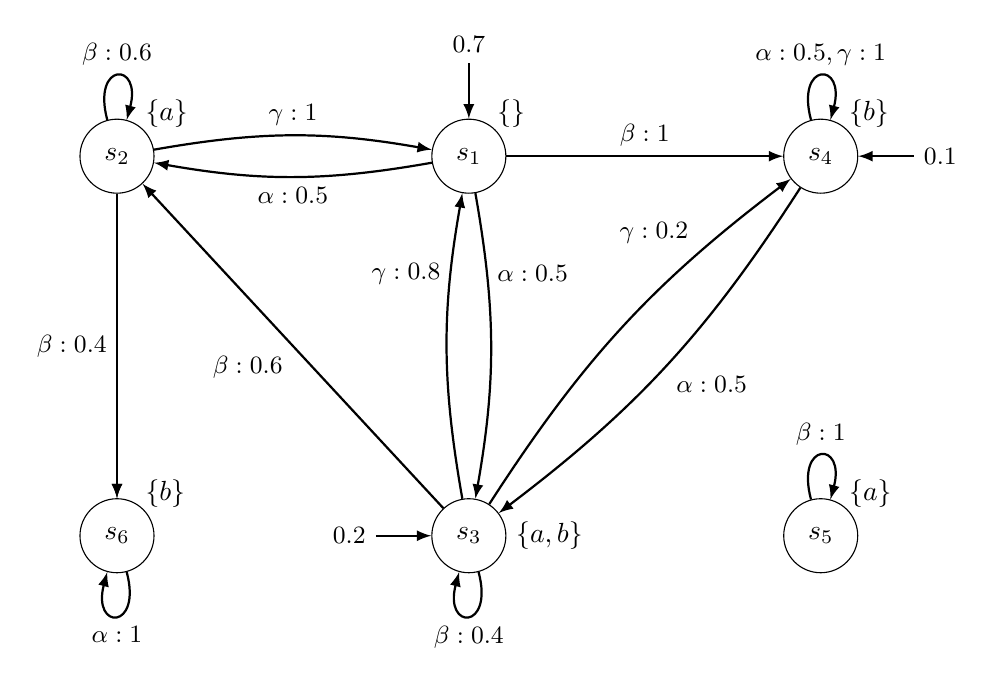
\begin{tikzpicture} [every initial by arrow/.style={thick}]
		\newcommand{\disthor}{100pt}
		\newcommand{\distvert}{110pt}
		%		\createstate{s1}{3,2+4}{$\state_1$};
		
		\node [mstate,initial above,initial text=\small$0.7$,initial distance=20pt] (s1) at (0,0) {$\state_1$};
		\node [mstate,left=\disthor of s1] (s2) {$\state_2$};
		\node [mstate,initial right	,initial text=\small$0.1$,initial distance=20pt,right=\disthor of s1] (s4) {$\state_4$};
		\node [mstate,initial left,initial text=\small$0.2$,initial distance=20pt,below=\distvert of s1] (s3) {$\state_3$};
		\node [mstate,mstate,initial above,initial text=,initial distance=20pt,left=\disthor of s3] (s6) {$\state_6$};
		\node [mstate,right=\disthor of s3] (s5) {$\state_5$};
	
		\path [trans] (s2) edge node [midway,left] {\small$\actionb: 0.4$} (s6);
		\path [trans] (s1) edge node [midway,above] {\small$\actionb: 1$} (s4);
		\path [trans] (s3) edge node [midway,below left] {\small$\actionb: 0.6$} (s2);
		
		\path [bendtrans] (s2) edge node [midway,above] {\small$\actionc: 1$} (s1);
		\path [bendtrans] (s1) edge node [midway,below] {\small$\action: 0.5$} (s2);

		\path [bendtrans] (s3) edge node [near end,left] {\small$\actionc: 0.8$} (s1);
		\path [bendtrans] (s1) edge node [near start,right] {\small$\action: 0.5$} (s3);

		\path [bendtrans] (s3) edge node [near end,above left] {\small$\actionc: 0.2$} (s4);
		\path [bendtrans] (s4) edge node [midway,below right] {\small$\action: 0.5$} (s3);
		
		\path [trans] (s2) edge [loop above] node [midway] {\small$\actionb:0.6$} (s2);
		\path [trans] (s3) edge [loop below] node [midway] {\small$\actionb:0.4$} (s3);
		\path [trans] (s4) edge [loop above] node [midway] {\small$\action:0.5, \actionc:1$} (s4);
		\path [trans] (s5) edge [loop above] node [midway] {\small$\actionb:1$} (s5);
		\path [trans] (s6) edge [loop below] node [midway] {\small$\action:1$} (s6);
		

		\node [above right=-4pt of s1] (ls1) {$\{\}$};
		\node [above right=-4pt of s2] (ls2) {$\{a\}$};
		\node [right=0pt of s3] (ls3) {$\{a,b\}$};
		\node [above right=-4pt of s4] (ls4) {$\{b\}$};
		\node [above right=-4pt of s5] (ls5) {$\{a\}$};
		\node [above right=-4pt of s6] (ls6) {$\{b\}$};

		
		
		
 	\end{tikzpicture}
\end{document}  
	\caption{Simplified representation of \mdp (left) and the \viewN \viewinitstates on it(left)}
	\label{fig:exampleMdp}  
\end{figure}
\end{exmp}

In the implementation and evaluation in chapters \ref{ch:viewimpl} and \ref{ch:eval} we will refer to \prism (PRobabilistIc Symbolic Model checker), which is why we will give a brief introduction on it. \prism is a model checker that can be used to define models and check them in an automated manner. In \prism a model is defined with modules, which interact with each other. A module consists of variables and commands. The (current) values of all the variables in the module define the (current) local state of the module. The global state of the model is defined by the local state of all modules.
%	\item Let in the following $x_1, \dots, x_l$ be variables of a module and $n_i$ the (current) value of $x_i$. The state of a module is defined by the value of its variables $(n_1, \dots, n_l)$
%	\item Let $\{y_1, \dots y_m\} \subseteq \{x_1, \dots, x_l\}$
A command in a module is of the form 
\[
\text{\texttt{[action] guard -> p\_1\!\;:\!\;update\_1\space+\space\dots\;\,+\space p\_m\!\;:\!\;update\_m;}} 
\]
where \texttt{p\_1, \dots\;\,, p\_m > 0} and \texttt{p\_1 + \dots\;\,+ p\_m = 1}.
The \texttt{guard} is a predicate on all variables of the model (including those of other modules). It may include operators such as negation (\texttt{!}), conjunction (\texttt{\&}) disjunction (\texttt{|}), arithmetic operators (\texttt{+}, \texttt{-}, \texttt{*}, \texttt{/}) or relational operators (\texttt{<}, \texttt{<=}, \texttt{>=}, \texttt{>}, \texttt{!=}, \texttt{=}, \texttt{=>}, \texttt{<=>}) as well as predefined functions.
An \texttt{update} represents a transition in the model which normally reflects a change of state. As a state is defined by the value of all the variables an update is specified by the assignment of new values to the variables of the module, possibly as a function of variables from other modules. The value of a variable remains unchanged, if it is not assigned a new value in an update. An update could look as follows:
\[
\text{\texttt{(x\_1'=1) \& (x\_2'=true) \& (x\_3'=0)}}
\]
This update assigns \texttt{1} to \texttt{x\_1}, \texttt{true} to \texttt{x\_2} and \texttt{0} to \texttt{x\_3}. In an update a variable is written in primed form (with $'$) to indicate that this will be the new value of that variable. Each assignment has to be in parentheses and separated with \texttt{\&} from other assignments.
The \texttt{action} can be included optionally for labeling the command or for synchronization purposes. In Listing \ref{lst:exmpprism} the model file for the \mdpN \mdp from Figure \ref{fig:exampleMdp} is shown. 
\begin{figure}
	\begin{lstlisting}[language=prism, caption={\prism model file for the \mdpN \mdp given by Figure \ref{fig:exampleMdp} \redcomment{initials not by probability!}. This example has only one variable representing the six states in \mdp and the actions \texttt{a}, \texttt{b} and \texttt{c} referring to \action, \actionb, and \actionc in \mdp, which are only used for labeling here.},label={lst:exmpprism}]
		mdp
		
		module onlymodule
		
		x : [1..6];
		
		[a] x=1 -> 0.5:(x'=2) + 0.5:(x'=3);
		[b] x=1 -> (x'=4);
		[b] x=2 -> 0.6:(x'=2) + 0.4:(x'=6);
		[c] x=2 -> (x'=1);
		[b] x=3 -> 0.4:(x'=3) + 0.6:(x'=2);
		[c] x=3 -> 0.8:(x'=1) + 0.2:(x'=4);
		[a] x=4 -> 0.5:(x'=4) + 0.5:(x'=3);
		[c] x=4 -> (x'=4);
		[b] x=5 -> (x'=5);
		[a] x=6 -> (x'=6);
		
		endmodule
		
		
		init
			x=1 | x=3 | x=4
		endinit		
	\end{lstlisting}
\end{figure}

Actions cause synchronization when included in several modules. If for example \texttt{action1} is included in two commands, which are in distinct modules these will be chosen simultaneously. If the guard of one of the commands with \texttt{action1} is not true, neither of the commands can be chosen\cite{Kwiatkowska2000, Kwiatkowska2011}.


%\redcomment{not sure if I should: $I := \initdistrib$ thereby meaning the underlying set}




\end{document}
 
